%%%%%%%%%%%%%%%%%%%%%%%%%%%%%%%%%%%%%%%%%%%%%%%%%%%%%%%%%%%%%%%%%%%%%%%%%%%
%                                                                         %
%		               SCHEDA LABORATORIO ALADDIN                         %
%			             ______________________                           %
%                                                                         %
%            			 AUTORE: Andrea Formica                           %
%                                                                         %
%			           Ultima revisione: 29.06.2018                       %
%                                                                         %
%%%%%%%%%%%%%%%%%%%%%%%%%%%%%%%%%%%%%%%%%%%%%%%%%%%%%%%%%%%%%%%%%%%%%%%%%%%
%
%
\documentclass[12pt]{article}
%
\usepackage[utf8]{inputenc}
\usepackage[english]{babel}
\usepackage{graphicx}
 
\setlength{\parindent}{2em}
\setlength{\parskip}{1em}

% per le accentate
\usepackage[utf8]{inputenc}
%
%
%			TITOLO
\title{Labirinti - tema informatico}
\author{A. Formica, G. Garbin, S. Patania}
%
\begin{document}
\maketitle
%
% 
\section{Introduzione}
Questo laboratorio ha come obiettivo l'introduzione degli studenti all'utilizzo dei costrutti iterativi e condizionali, utilizzati nei linguaggi di programmazione, attraverso un ambiente di programmazione visuale. Grazie ai linguaggi di programmazione possiamo scrivere dei programmi che automatizzano la risoluzione di un problema. La conoscenza delle strutture iterative e condizionali permette di scrivere un programma più compatto e semplice da leggere.
%
%
\section{Costrutti iterativi}
Consideriamo il labirinto \figurename~\ref{fig:maze_iter}: il programma più semplice che viene in mente per risolverlo è quello mostrato nella \figurename~\ref{fig:sol_non_iter}. Osservando la soluzione proposta possiamo notare che le prime quattro istruzioni si ripetono per quattro volte nello stesso ordine. I linguaggi di programmazione mettono quindi a disposizione dei costrutti che permettono di ripetere \textit{n} volte un blocco di istruzioni. Grazie a questa primitiva possiamo semplificare la soluzione precedente scrivendo un'unica volta la parte di codice che si ripete, come mostrato nella \figurename~\ref{fig:sol_iter}. Nei linguaggi di programmazione tale costrutto viene chiamato \textit{ciclo for}. Nell'attività dei robot troviamo un costrutto iterativo nel superpotere RIPETI $\langle$n$\rangle$ VOLTE $\langle$post-it$\rangle$.
 
\begin{figure}
\centering

\includegraphics[scale=0.35]{img/maze3.jpg}
\caption{Labirinto risolvibile con costrutto iterativo}
\label{fig:maze_iter}
\end{figure}

\begin{figure}
\centering
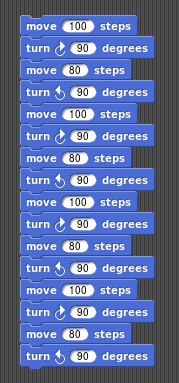
\includegraphics[scale=0.7]{img/non_iter.jpg}
\caption{Soluzione senza costrutto iterativo}
\label{fig:sol_non_iter}
\end{figure}

\begin{figure}
\centering
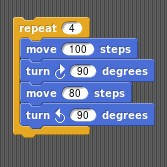
\includegraphics[scale=0.7]{img/loop.jpg}
\caption{Soluzione con costrutto iterativo}
\label{fig:sol_iter}
\end{figure}
%
%
\section{Costrutti condizionali}
I costrutti condizionali permettono di eseguire una o più istruzioni al verificarsi di una determinata condizione. Il codice mostrato nella \figurename~\ref{fig:if} utilizza tale costrutto: se è vera la condizione dell'if allora verrà eseguita l'istruzione del ramo \textit{if}, se invece è falsa viene eseguita l'istruzione nel ramo \textit{else}. Questo costrutto permette perciò di modificare il flusso di esecuzione del programma al verificarsi di determinate condizioni. Nei linguaggi di programmazione questa struttra di controllo viene chiamata \textit{if-else}. Nell'attività dei robot, il superpotere SE $\langle$condizione$\rangle$ ESEGUI $\langle$post-it$\rangle$ corrisponde a un costrutto condizionale (in cui non è presente il ramo \textit{else}).

\begin{figure}
\centering
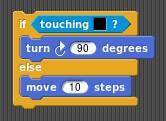
\includegraphics[scale=0.7]{img/if.jpg}
\caption{Costrutto condizionale}
\label{fig:if}
\end{figure}
%
%
\section{Costrutti condizionali e iterativi}
Nei linguaggi di programmazione esiste anche una primitiva che combina i costrutti iterativi con quelli condizionali, come si può vedere nella \figurename~\ref{fig:while}. Tale costrutto permette di ripetere un blocco di istruzioni fino a che si verifica una determinata condizione. Nei linguaggi di programmazione questo costrutto si traduce nei cicli \textit{while} e \textit{do-while}. Nell'attività dei robot, ritroviamo questo costrutto nel superpotere: RIPETI FINO A QUANDO $\langle$condizione$\rangle$:  $\langle$post-it$\rangle$.

\begin{figure}
\centering
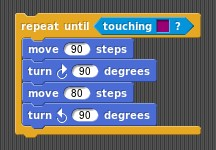
\includegraphics[scale=0.7]{img/while.jpg}
\caption{Costrutto iterativo e condizionale}
\label{fig:while}
\end{figure}
\end{document}